%%%%%%%%%%%%%%%%%%%%%%%%%%%%%%%%%%%%%%%%%%%%%%%%%%%%%%%%%%%%%%%%%%%%%%%%%%%%
% AGUtmpl.tex: this template file is for articles formatted with LaTeX2e,
% Modified March 2013
%
% This template includes commands and instructions
% given in the order necessary to produce a final output that will
% satisfy AGU requirements.
%
% PLEASE DO NOT USE YOUR OWN MACROS
% DO NOT USE \newcommand, \renewcommand, or \def.
%
% FOR FIGURES, DO NOT USE \psfrag or \subfigure.
%
%%%%%%%%%%%%%%%%%%%%%%%%%%%%%%%%%%%%%%%%%%%%%%%%%%%%%%%%%%%%%%%%%%%%%%%%%%%%
%
% All questions should be e-mailed to latex@agu.org.
%
%%%%%%%%%%%%%%%%%%%%%%%%%%%%%%%%%%%%%%%%%%%%%%%%%%%%%%%%%%%%%%%%%%%%%%%%%%%%
%
% Step 1: Set the \documentclass
%
% There are two options for article format: two column (default)
% and draft.
%
% PLEASE USE THE DRAFT OPTION TO SUBMIT YOUR PAPERS.
% The draft option produces double spaced output.
%
% Choose the journal abbreviation for the journal you are
% submitting to:

% jgrga JOURNAL OF GEOPHYSICAL RESEARCH
% gbc   GLOBAL BIOCHEMICAL CYCLES
% grl   GEOPHYSICAL RESEARCH LETTERS
% pal   PALEOCEANOGRAPHY
% ras   RADIO SCIENCE
% rog   REVIEWS OF GEOPHYSICS
% tec   TECTONICS
% wrr   WATER RESOURCES RESEARCH
% gc    GEOCHEMISTRY, GEOPHYSICS, GEOSYSTEMS
% sw    SPACE WEATHER
% ms    JAMES
% ef    EARTH'S FUTURE
%
%
%
% (If you are submitting to a journal other than jgrga,
% substitute the initials of the journal for "jgrga" below.)

\documentclass[draft,gc]{AGUTeX}
% To create numbered lines:

% If you don't already have lineno.sty, you can download it from
% http://www.ctan.org/tex-archive/macros/latex/contrib/ednotes/
% (or search the internet for lineno.sty ctan), available at TeX Archive Network (CTAN).
% Take care that you always use the latest version.

% To activate the commands, uncomment \usepackage{lineno}
% and \linenumbers*[1]command, below:
%\usepackage{natbib} 
\usepackage{lineno}
\linenumbers*[1]

%  To add line numbers to lines with equations:
%  \begin{linenomath*}
%  \begin{equation}
%  \end{equation}
%  \end{linenomath*}
%%%%%%%%%%%%%%%%%%%%%%%%%%%%%%%%%%%%%%%%%%%%%%%%%%%%%%%%%%%%%%%%%%%%%%%%%
% Figures and Tables
%
%
% DO NOT USE \psfrag or \subfigure commands.
%
%  Figures and tables should be placed AT THE END OF THE ARTICLE,
%  after the references.
%
%  Uncomment the following command to include .eps files
%  (comment out this line for draft format):
\usepackage{graphicx}
%
%  Uncomment the following command to allow illustrations to print
%   when using Draft:
\setkeys{Gin}{draft=false}
%
% Substitute one of the following for [dvips] above
% if you are using a different driver program and want to
% proof your illustrations on your machine:
%
% [xdvi], [dvipdf], [dvipsone], [dviwindo], [emtex], [dviwin],
% [pctexps],  [pctexwin],  [pctexhp],  [pctex32], [truetex], [tcidvi],
% [oztex], [textures]
%
% See how to enter figures and tables at the end of the article, after
% references.
%
%% ------------------------------------------------------------------------ %%
%
%  ENTER PREAMBLE
%
%% ------------------------------------------------------------------------ %%

% Author names in capital letters:
\authorrunninghead{SWANSON-HYSELL ET AL.}

% Shorter version of title entered in capital letters:
\titlerunninghead{SIGNIFICANT PLATE MOTION DURING RIFT DEVELOPMENT}

%Corresponding author mailing address and e-mail address:
%\authoraddr{Corresponding author: N. L. Swanson-Hysell,
%Department of Earth and Planetary Science, University of
%California, Berkeley, CA 94720, USA.
%(swanson-hysell@berkeley.edu)}

\begin{document}

%% ------------------------------------------------------------------------ %%
%
%  TITLE
%
%% ------------------------------------------------------------------------ %%


\title{Confirmation of progressive plate motion during the Midcontinent Rift's early magmatic stage from the Osler Volcanic Group, Ontario, Canada}

%% ------------------------------------------------------------------------ %%
%
%  AUTHORS AND AFFILIATIONS
%
%% ------------------------------------------------------------------------ %%


%Use \author{\altaffilmark{}} and \altaffiltext{}

% \altaffilmark will produce footnote;
% matching \altaffiltext will appear at bottom of page.

\authors{Nicholas. L. Swanson-Hysell,\altaffilmark{1,2} Angus A. Vaughan,\altaffilmark{1,3}, Monica R. Mustain,\altaffilmark{1,4} and Kristofer E. Asp\altaffilmark{1,5}}

\altaffiltext{1}{Institute for Rock Magnetism, Department of Earth Sciences, University of Minnesota, Minneapolis, Minnesota, USA}

\altaffiltext{2}{Department of Earth and Planetary Science, University of California, Berkeley, California, USA}

\altaffiltext{3}{Department of Geology, Carleton College, Northfield, Minnesota, USA}

\altaffiltext{4}{Department of Geology and Geography, Illinois State University, Normal, Illinois, USA}

\altaffiltext{5}{Department of Geological Sciences, University of Minnesota, Duluth, Minnesota, USA}

%% ------------------------------------------------------------------------ %%
%
%  ABSTRACT
%
%% ------------------------------------------------------------------------ %%

% >> Do NOT include any \begin...\end commands within
% >> the body of the abstract.

\begin{abstract}
As the supercontinent Rodinia was assembling ca. 1.1 billion years ago, there was extensive magmatism on at least five Proterozoic continents including the development of the North American Midcontinent Rift. New paleomagnetic data from 84 lava flows of the Osler Volcanic Group of the Midcontinent Rift reveal that there was a significant and progressive decrease in inclination between the initiation of extrusive volcanism in the region (ca. 1110 Ma) and ca. 1105 $\pm$ 2 Ma (the ``early stage" of rift development). Paleomagnetic poles can be calculated for the lower portion of the reversed Osler Volcanic Group (40.9$^\circ$N, 218.6$^\circ$E, A$_{95}$=4.8$^\circ$, N=30)  and the upper portion of the reversed Osler Volcanic Group (42.5$^\circ$N, 201.6$^\circ$E, A$_{95}$=3.7$^\circ$, N=59; this pole can be assigned the age of ca. 1105 $\pm$ 2 Ma). This result is a positive test of the hypothesis that there was significant plate motion during the early stage of rift development. In addition to being a time of widespread volcanism on Laurentia and other continents, this interval of the late Mesoproterozoic was characterized by rapid paleogeographic change.
\end{abstract}

%% ------------------------------------------------------------------------ %%
%
%  BEGIN ARTICLE
%
%% ------------------------------------------------------------------------ %%

% The body of the article must start with a \begin{article} command
%
% \end{article} must follow the references section, before the figures
%  and tables.

\begin{article}

%% ------------------------------------------------------------------------ %%
%
%  TEXT
%
%% ------------------------------------------------------------------------ %%

\section{Introduction}
Despite being active for more than 20 million years \citep{Davis1997a} and resulting in the thinning of pre-rift crust to less than 10 km \citep{Cannon1992b}, the 1.1 Ga Midcontinent Rift failed to dismember the Laurentian craton. This failure resulted in the preservation of a thick record of rift-related volcanic and sedimentary rocks that gives geoscientists insight into the development of this ancient rift. Most models for the development of the Midcontinent Rift attribute its origin to the upwelling and decompression melting of a mantle plume \citep{Shirey1997a}. On the basis of the great volume of generated magma and interpretation of geochemical data, it is argued that the early stage plateau flood basalts of the rift (ca. 1110-1105 Ma) and the main stage volcanics that erupted into the central basin (ca. 1100-1095 Ma) were both dominated by plume-sourced melts. This deep-plume origin for the rift needs to be considered in conjunction with paleogeographic change that has been inferred to have been ongoing throughout rift development. Fully constraining this paleogeographic change is essential for understanding rift development and for constraining late Mesoproterozoic paleogeographic reconstructions given the centrality of Laurentia's apparent polar wander path to such efforts.

It has long been noted that there is a significant difference in paleomagnetic inclination between the steep (dominantly reversed polarity) magnetizations of the oldest volcanics and intrusives of the Midcontinent Rift and the shallower (dominantly normal polarity) magnetizations from the younger main stage volcanics and intrusives \citep{Halls1982a}. This inclination change has been interpreted either as resulting from rapid plate motion \citep{Robertson1971a, Davis1997a} or as being the result of large non-dipolar contributions to the late Mesoproterozoic geomagnetic field that led to asymmetry across reversals \citep{Pesonen1981a}. The interpretation of the record as recording stepwise inclination change across reversals associated with a significant sustained departure from a geocentric axial dipole (GAD) dominated field was challenged by the observation of a progressive decrease in paleomagnetic inclination across multiple geomagnetic reversals up through the succession of Midcontinent Rift lavas at Mamainse Point, Ontario \citep{Swanson-Hysell2009a, Swanson-Hysell2014a}. This progressive decrease in inclination leads to the interpretation of multiple symmetric reversals when the data are considered in stratigraphic context and these results have been used to support the hypothesis that rapid paleogeographic change was ongoing during Midcontinent Rift magmatism \citep{Buchan2013a, Swanson-Hysell2014a}. To date, Mamainse Point is the only succession where a progressive decrease in inclination through an exposure of rift stratigraphy has been reported. At Mamainse Point, much of the decrease in paleomagnetic inclination occurs within the lowermost reversed polarity portion of the stratigraphy that erupted during the early magmatic stage of rift development \citep{Swanson-Hysell2014a}. This result sets up the prediction that other localities in the rift that span the same period of time should also record such a decrease. This work tests that hypothesis with new paleomagnetic data developed in stratigraphic context from the Osler Volcanic Group. 

\section{Geology and context of the Osler Volcanic Group}
\subsection{Osler Volcanic Group lithologies}
The Osler Volcanic Group overlies the epicontinental sediments of the Mesoproterozoic Sibley Group. The lowest 100 meters of the Osler Volcanic Group contains rift-related sandstones and conglomerates \citep{Hollings2007a}, which are followed by a succession of relatively continuous tholeiitic basalt flows. We studied these flows along the east shore of Simpson Island in the Lake Superior Archipelago. This location has well-preserved basalt flows and exposure of a significant thickness of the Osler Volcanic Group stratigraphy. This location occurs at a great enough distance ($>$ 10 km) from the intrusive St. Ignace Island Complex so that the magnetizations of the flows are apparently unaffected by its emplacement. The St. Ignace Island Complex is dominated by felsic lithologies and was emplaced into the mafic flows of the Osler Volcanic Group near the end of Midcontinent Rift volcanism \citep{Hollings2007b}.

Along the east shore of Simpson Island, where we measured stratigraphic sections (Fig. \ref{fig:map}), the stratigraphic succesion is dominated by basaltic lava flows with typical thicknesses of ca. 5 meters. For the 105 flows in the measured stratigraphic sections (that represent a subset of the total stratigraphy) where there is sufficient exposure of the flow base, interior and top to determine thickness, the median flow thickness is 4.9 meters with a first quartile thickness of 2.0 meters and third quartile thickness of 9.8 meters (details are provided in the supporting information). Minor interflow siltstone and conglomerate occur between some flows and provide constraints on paleo-horizontal that were utilized for structural corrections of paleomagnetic data (Fig. \ref{fig:map}). The red-brown siltstone beds are generally centimeters to tens of centimeters thick while the conglomerate beds can be up to several meters in thickness. Clasts in the conglomerate beds are basaltic in composition and are primarily pebble-sized, but can range up to 10 cm in diameter. Within the stratigraphic sections, individual flows can be distinguished by their characteristic transition in texture moving up through the flow: pipe vesicles at the base of flows, to massive basalt, to massive basalt with some amygdules, to a highly amygdaloidal texture at the top of the flows. There is well-preserved pahoehoe flow-banding on some flow tops. Using our measurements of bedding orientation, we estimate that slightly over 3000 meters of the Osler Volcanic Group is exposed on Simpson Island (Fig. \ref{fig:map}).

\subsection{Angular unconformity and associated paleomagnetic reversal}

Southwest of Simpson Island in the Nipigon Strait region there is exposure on Puff Island, which contains an angular unconformity marked by a conglomerate that separates underlying flows of reversed magnetic polarity from overlying flows of normal magnetic polarity \citep{Halls1974a}. This unconformity is stratigraphically higher than the top of the exposure at Simpson Island where all studied flows have reversed magnetic polarity. Only ca. 110 stratigraphic meters of normally magnetized flows are exposed south (i.e. stratigraphically above) of the unconformity on Puff Island before the sequence is covered by Lake Superior. This unconformity has been interpreted to be due to a period of quiescence of local volcanism \citep{Halls1974a}. \citet{Halls1974a} was the first to suggest that such quiescence may have been widespread throughout the Midcontinent Rift---an idea that is now incorporated into models of rift development that utilize interpretations of the distribution of U-Pb dates and has been termed the ``latent stage" \citep{Vervoort2007a}. As occurs in sequences across the Midcontinent Rift, the lower reversed flows studied paleomagnetically by \citet{Halls1974a} have a steeper inclination, in an absolute sense, than the younger normal flows above the unconformity. The missing time evidenced by the angular unconformity likely correlates with the missing time inferred from radiometric dates on units within the North Shore Volcanic Group and the Powder Mill Group \citep{Davis1997a, Zartman1997a}. In these rift successions, the stratigraphic intervals where time is inferred to be missing are associated with a switch from reversed to normal magnetic polarity. A new U-Pb date from Mamainse Point (1100.36 $\pm$ 0.25 Ma from the upper reversed polarity zone) demonstrates that, in contrast to successions with missing time or condensed stratigraphy, the sequence there is relatively complete thereby preserving additional geomagnetic reversals \citep{Swanson-Hysell2014a}. 

%Used Halls (1974) map to determine placement of unconformity and that ca. 630 meters of horizontal exposure exists above it. Using the dip of 10º shown on the Halls map determined the thickness to be ~110 meters per the IPython code below:
%In [20]: def deg2rad(degrees):
%        pi = math.pi
%        radians = pi * degrees / 180
%        return radians
%   ....: 
%
%In [21]: angle = deg2rad(10)
%
%In [22]: strat = math.sin(angle)*630
%
%In [23]: print strat
%109.39835193

The paleomagnetic data that \citet{Halls1974a} developed from Osler Volcanic Group flows were in relatively close stratigraphic proximity below and above the unconformity (as the goal of the study was to confirm the presence of a geomagnetic reversal that had been inferred from aeromagnetic data; \cite{Halls1972a}). The aeromagnetic data demonstrated that the reminder of the flows below the unconformity (i.e. to the north) and stratigraphically below those studied by \citet{Halls1974a} are also of reversed magnetic polarity. On the basis of polarity and the geochronology discussed below, the interval has been correlated with the ``early stage" of Midcontinent Rift development and the other basal sequences of lava flows within the rift. These early stage flows are interpreted to be plateau lavas that erupted over a broad geographic area prior to significant development of the main central rift graben that underlies present day Lake Superior \citep{Cannon1992b}. Due to being limited to the portion of the succession in close stratigraphic proximity to the angular unconformity, existing data have not permitted evaluation of whether or not there is a progressive change in paleomagnetic inclination through the reversed polarity flows as observed in the ``early stage" volcanics at Mamainse Point \citep{Swanson-Hysell2009a}.

\subsection{Age constraints on the Osler Volcanic Group}

In some locales, a quartz-feldspar, porphyritic felsic unit occurs near the base of the Osler Volcanic Group for which a U-Pb zircon date of 1107.5$^{+4}_{-2}$ Ma has been reported \citep{Davis1985a}.  This date was obtained from an outcrop of felsic porphyry on Black Bay Peninsula, ca. 40 km to the west of Simpson Island \citep{Davis1985a}.  This unit was tentatively interpreted as extrusive \citep{Davis1985a, Lightfoot1991a} and the date has been interpreted as constraining the time at which Osler Group volcanism commenced.  New observations made of a quartz-feldspar porphyry unit on Simpson Island, mapped as equivalent to the unit from which the date was obtained \citep{Giguere1975a}, provide additional evidence for the inference made by \citet{Giguere1975a} that this unit is actually intrusive.  On Simpson Island, the basal sedimentary units of the Osler Volcanic Group are overlain by the quartz-feldspar porphyry which itself underlies the basalt flows (Fig. \ref{fig:map}). A thin (1-2 mm thick) veneer of basalt is variably present overlying the porphyry.  The basalt veneer displays pahoehoe flow banding, which is unlikely to have developed if the flow was originally this thin, implying that the felsic unit intruded into the basalt, cutting into an originally thicker flow.  An additional observation is that there are protrusions of porphyry surrounded by host basalt, providing further support for an intrusive relationship. If the Simpson Island intrusion is indeed equivalent to the Black Bay Peninsula unit, this evidence suggests that the  1107.5$^{+4}_{-2}$ Ma  date is a minimum age for the eruption of the first Osler basalt flows, rather than an absolute age for that point in the Osler Volcanic Group stratigraphic succession. This unit should be a target for future geochronology.

A sequence of quartz-feldspar phyric rhyolite flows occurs near the top of the magnetically reversed portion of the Osler Volcanic Group at Agate Point (\cite{Davis1985a}; Fig. \ref{fig:summary}; stratigraphically higher than the highest flow on Simpson Island). \cite{Davis1997a} obtained a U-Pb zircon date from the Agate Point Rhyolite of 1105 $\pm$ 2 Ma which, if the extrusive interpretation is correct, is a robust age for that point in the Osler Volcanic Group stratigraphy.

\section{Methods}

We collected oriented samples for magnetic laboratory measurements during the course of measuring stratigraphic sections (Fig. \ref{fig:map}). Each site consists of an individual lava flow from which we collected 6 to 10 small (2 cm diameter) rock cores with a hand-held drill. These small core samples were oriented with a magnetic and sun compass, when possible, such that their spatial orientation is known. To minimize the visual impact of collecting these small cores along the pristine Lake Superior shoreline, we knocked out the portion of the outcrop from which they were collected.

At the Institute for Rock Magnetism, specimens were prepared from the samples and subjected to progressive thermal or alternating field (AF) demagnetization (Fig \ref{fig:pmagrockmag}A). Initial results on sister specimens demonstrated the simplicity of the magnetizations and the similarity between results obtained through thermal and AF demagnetization (Fig \ref{fig:pmagrockmag}A). Low-temperature remanence experiments were run on representative samples and loss of remanence across the Verwey transition demonstrates that the magnetic mineralogy is dominated by low-titanium magnetite (e.g. Fig \ref{fig:pmagrockmag}B). These results revealed the ability of AF demagnetization to isolate the characteristic remanent magnetization (ChRM) held by magnetite with relatively small and variably present overprints being effectively removed by low-field AF steps. Given these results, the majority of flows were studied with AF demagnetization alone.

%The first section (SI1) was started at the base of the lowest Osler flow exposed on the eastern shore of Simpson Island above the felsic porphyry and comprises 143 meters of stratigraphic height. Three more sections were measured along the eastern shore (SI2, SI3, and SI4) with SI4 ending at Morn Point on the southeastern tip of the island. SI2 consisted of three separate subsections (SI2a, SI2b, SI2c) that were separated by significant amounts of cover, and comprise 14 meters, 12 meters, and 33 meters of stratigraphic height, respectively. SI3 and SI4 comprise 130 and 40 meters of stratigraphy, respectively. Section SI5 was measured on the southern end of Simpson Island, and consists of subsections SI5b (217 meters of stratigraphy ending at Grebe Point) and SI5a (one thick flow measured on an island right offshore of Grebe Point, and the highest measured flow in the stratigraphic succession).

\section{Results and Discussion}

Flow means from the data generated for 84 flows of the Osler Volcanic Group are summarized in Figures \ref{fig:map} and \ref{fig:summary} and in a table in the supporting information. To consider whether the flows of the Osler Volcanic Group record progressive paleogeographic change, we take the approach of grouping and comparing data from the lower third of the sequence (0 to 1041 meters; 30 flows), the middle third of the sequence (1041 to 2083 meters; 20 flows) and the upper third of the sequence (2083 to 3124 meters; 34 flows). To test whether these subsets of the data could have been drawn from a common mean, we apply both the Watson V$_{\mathrm w}$ test with Monte Carlo simulation \citep{Watson1983a} and the bootstrap test for a common mean \citep{Tauxe2010a}. Full details associated with these statistical tests are provided in the supporting information. The results from these common mean statistical tests show that the directions from the lower third of the sequence cannot be distinguished from those from the middle third, nor can the directions from the upper third of the sequence be distinguished from those in the middle third. In contrast, directions from the lower third of the sequence can be distinguished from those of the upper third at the 95$\%$ confidence level. This result can be seen visually in Figure \ref{fig:summary} as the $\alpha_{95}$ ellipses associated with the directional means and the A$_{95}$ ellipses associated with the pole means do not overlap. The statistically significant difference between the populations of flow means in the lower and upper third of the stratigraphy, combined with the result that the middle third data has a mean that is an intermediate direction between the lower and upper means, supports the hypothesis that progressive plate motion was ongoing throughout the eruption of the Osler Volcanic Group with Laurentia moving to lower latitudes (see reconstruction Fig. \ref{fig:summary}). The paleomagnetic poles calculated and used in the paleogeographic reconstruction in Fig. \ref{fig:summary} are: lower third Simpson Island Osler Group (40.9$^\circ$N, 218.6$^\circ$E, A$_{95}$=4.8$^\circ$, N=30); middle third Simpson Island Osler Group (42.7$^\circ$N, 211.3$^\circ$E, A$_{95}$=8.2$^\circ$, N=20)  and the upper portion of the reversed Osler Group (41.6$^\circ$N, 205.4$^\circ$E, A$_{95}$=4.8$^\circ$, N=34). Stratigraphic subgroups of the Simpson Island data can be made in many different ways than this approach of dividing the stratigraphic sequence into thirds. For example, comparing the 17 flows in the lowermost 500 meters against the 17 flows in the uppermost 500 meters, demonstrates that those populations are dramatically different such that the bootstrap test for a common mean shows their x, y and z components to be distinct at the 99$\%$ confidence level (see supporting information for details). Comparing the 41 flows in the lower half of the stratigraphic succession to the 43 flows in the upper half of the stratigraphic succession also reveals a statistically significant, but relatively small, difference between the populations (see supporting information for details). We focus on the lower, middle and upper third grouping in our analysis making the judgement that such an analysis strikes the balance between considering the possibility of change through the stratigraphy while binning enough data over thick enough intervals to not to be significantly biased by under-averaging secular variation. In this grouping, each bin contains $>$100 meters of relatively thin pahoehoe basalt flows.

The paleomagnetic data developed by \citet{Halls1974a} come from the Osler Volcanic Group in the Nipigon Straits region. The data were obtained from the uppermost part of the stratigraphic succession below the angular unconformity on Puff Island that separates the flows of reversed polarity from younger flows of normal polarity. The \citet{Halls1974a} data of reversed polarity (N=25,  http://earthref.org/MAGIC/9518) comes from a portion of the stratigraphy that should correlate with the upper third of the sequence at Simpson Island. Given that the flows are dominantly thin pahoehoe lavas and that the \citet{Halls1974a} study area was ca. 30 km eastward in the vicinity of the Nipigon Strait, those data should be comprised of distinct individual cooling units from the Simpson Island flows. Watson and bootstrap tests for a common mean between the \citet{Halls1974a} data of reversed polarity and data from the upper third of the stratigraphy at Simpson Island are positive indicating that the populations of directions cannot be distinguished from one another---consistent with this stratigraphic correlation. In contrast, tests for a common mean between the reversed polarity \citet{Halls1974a} data and the lower third of the Simpson Island stratigraphy fail. This result indicates that the populations are statistically distinct, building on the result that there was significant paleogeographic change recorded by the Osler Volcanic Group. Given that the data from the upper third of the stratigraphy on Simpson Island correlate stratigraphically and share a common mean with the Halls (1974) data from the Nipigon Straits region, we can calculate a mean paleomagnetic pole for the upper portion of the reversed Osler Volcanic Group stratigraphy (42.5$^\circ$N, 201.6$^\circ$E, A$_{95}$=3.7$^\circ$, N=59). This pole can be assigned an approximate age of 1105 $\pm$ 2 Ma using the date from the Agate Point rhyolite \citep{Davis1997a}.

These new data from 84 flows of Osler Volcanic Group from the early stage of the Midcontinent Rift bolster evidence from the succession at Mamainse Point that the decrease in inclination through the history of the rift is a progressive change rather than a step-wise change across reversals. The interpretation of a step-wise change of inclination across reversals has been used to argue for reversal asymmetry at the time that was proposed to result from significant deviation from an axial dipole geomagnetic field \citep{Pesonen1981a}. The observed progressive change in inclination is more consistent with the hypothesis that inclination decrease is a result of fast equatorward motion of Laurentia \citep{Davis1997a, Swanson-Hysell2009a}. The poles calculated from the stratigraphic groupings of the Osler Volcanic Group at Simpson Island fit the progression along the path suggested by paleomagnetic poles from the lowermost polarity zone at Mamainse Point, Ontario. These data sets combined indicate that there was significant plate motion during the early magmatic stage of North American Midcontinent Rift development. \textit{\textbf{This text it still a work in progress: At present, the duration of Osler Volcanic GRoup volcanism remains poorly constrained given the uncertainties on the ages and the lack of a dated unit that can firmly be demonstrated to be extrusive near the base of the group. This reality makes it difficult to go from the plate motion inferred from the Osler Volcanic Group poles to a rate estimate based on that motion alone. What can be done is to develop a rate estimate from}}

%48.3º paleolatitude for Lake Superior Archipelago implied by lower 1/3 Simpson Island pole
%23.6º paleolatitude for Lake Superior Archipelago implied by lower Portage Lake Volcanics pole

From the beginning of Midcontinent Rift extrusive volcanism in the early magmatic stage (ca. 1110 to 1105 Ma) to the voluminous volcanism associated with the main magmatic stage of rift development (ca. 1100 to 1095 Ma) there was ca. 25$^\circ$ of latitudinal motion of North America. The voluminous volcanism appears to have been concentrated in the Lake Superior region both during the early magmatic stage and during the eruption of the thick main stage volcanics in the central graben. Arguments for a plume-origin for Midcontinent Rift volcanism have argued that a plume is necessary to explain isotopic signatures in lava flows (Nd isotopes, \citet{Nicholson1997a}; Re-Os data, \citet{Shirey1997a}) and as a heat source for generating the large volumes of basaltic magma associated with the rift \citep{Cannon1992b}. If a long-lived plume was in a fixed position relative to Earth's spin axis and did not become significantly diverted upon reaching the lithosphere, large relative motion of Laurentia would make it unable to continue to be a source of melt to the rift. One possibility is that the North American plate and a deep-seated mantle plume traveled in unison to lower latitudes as a result of large-scale rapid true polar wander. The motion implied by Keweenawan Track poles has been interpreted as a result of true polar wander \citep{Evans2003b, Mitchell2012a}. To reconcile an interpretation of rapid plate motion through differential plate tectonic motion, rather than true polar wander with a continued plume contribution, \citet{Davis1997a} proposed that a plume head drifted with continental lithosphere. This idea can be considered in the context of the model of ``upside-down drainage" for positively buoyant plume material wherein relief at the base of the lithosphere directs lateral flow \citep{Sleep1997a, Ebinger1998a}. Given the significant lithospheric thinning associated with rifting, plume material could continue to be directed into the rift sustaining magmatism despite ongoing plate motion.

At the same time that the Midcontinent Rift was initiating in Laurentia the following igneous provinces were emplaced on four other cratons:
\begin{itemize}
\item the Umkondo large igneous province of the Kalahari Craton (many ID-TIMS U-Pb dates on zircon and baddeleyite between 1112 and 1108 Ma; \cite{Hanson2004a})
\item  thick and extensive gabbro-norite (GN) dikes exposed in the southwest Angola portion of the Congo Craton (one of which has an ID-TIMS U-Pb date on baddeleyite of 1110.3 $\pm$ 2.5 Ma; \cite{Ernst2013a})
\item the Mahoba suite of dikes of the India Craton (one of which, the ``Great Dike of Mahoba" has an laser ablation U-Pb date on zircon of 1112.7 $\pm$ 7.4 Ma; \cite{Pradhan2012a})
\item a putative ca. 1110 Ma large igneous province in the southwest portion of the Amazonia craton inferred from dates on two widely separated intrusions (ID-TIMS U-Pb date on baddeleyite from the Rinc\'on del Tigre intrusion of 1110.4 $\pm$ 1.8 Ma and a sill within Aguepe\'i sediments with a ID-TIMS U-Pb date on baddeleyite of 1111.5 $\pm$ 1.5 Ma \cite{Hamilton2012a})
\end{itemize}

This contemporaneous voluminous volcanism on five late Mesoproterozoic cratons is coincident with the onset of Laurentia's rapid plate motion. This temporal correlation suggests that this time period was characterized by particularly vigorous plume activity, that in addition to large igneous province development may be connected to the driving forces that resulted in rapid plate motion and/or true polar wander.

\section{Conclusion}

Lava flows of the Osler Volcanic Group below the Puff Island unconformity erupted during the early magmatic stage of Midcontinent Rift development during a time interval characterized by reversed magnetic polarity. New paleomagnetic data from 84 Osler Volcanic Group lava flows reveal a significant decrease in paleomagnetic inclination through the sequence of lava flows. These results support the hypothesis that the difference between the steep paleomagnetic inclinations characteristic of the early magmatic stage and the relatively shallower inclinations of the main magmatic stage throughout the rift are the result of rapid plate motion that was recorded by the Osler Volcanic Group.

%%% End of body of article:

%%%%%%%%%%%%%%%%%%%%%%%%%%%%%%%%
%% Optional Appendix goes here
%
% \appendix resets counters and redefines section heads
% but doesn't print anything.
% After typing \appendix
%
%\section{Here Is Appendix Title}
% will show
% Appendix A: Here Is Appendix Title
%
%%%%%%%%%%%%%%%%%%%%%%%%%%%%%%%%%%%%%%%%%%%%%%%%%%%%%%%%%%%%%%%%
%
% Optional Glossary or Notation section, goes here
%
%%%%%%%%%%%%%%
% Glossary is only allowed in Reviews of Geophysics
% \section*{Glossary}
% \paragraph{Term}
% Term Definition here
%
%%%%%%%%%%%%%%
% Notation -- End each entry with a period.
% \begin{notation}
% Term & definition.\\
% Second term & second definition.\\
% \end{notation}
%%%%%%%%%%%%%%%%%%%%%%%%%%%%%%%%%%%%%%%%%%%%%%%%%%%%%%%%%%%%%%%%
%
%  ACKNOWLEDGMENTS

\begin{acknowledgments}
The Ontario Ministry of Natural Resources granted permits for work to be conducted in the Lake Superior Archipelago Conservation Reserve. Pete Hollings of Lakehead University along with Dorothy Campbell and John Scott of the Ontario Geological Survey provided an introduction to the geology of the Lake Superior Archipelago. This work benefitted from discussions with Robert Cundari, Josh Feinberg and Henry Halls. Reviews from Trond Torsvik and an anonymous referee lead to significant improvements of the manuscript. Julie Bowles, Mike Jackson and Peat Solheid provided support for measurements at the Institute for Rock Magnetism. This research was supported by NSF EAR-1045635 to N.L.S.-H. and the NSF-funded Research Experiences for Undergraduates program in the Department of Earth Sciences at the University of Minnesota that supported A.A.V. and M.R.M.. This is IRM contribution $\#$1312.

\end{acknowledgments}

%% ------------------------------------------------------------------------ %%
%%  REFERENCE LIST AND TEXT CITATIONS
%
% Either type in your references using
% \begin{thebibliography}{}
% \bibitem{}
% Text
% \end{thebibliography}
%
% Or,
%
% If you use BiBTeX for your references, please use the agufull08.bst file (available at % ftp://ftp.agu.org/journals/latex/journals/Manuscript-Preparation/) to produce your .bbl
% file and copy the contents into your paper here.
%
% Follow these steps:
% 1. Run LaTeX on your LaTeX file.
%
% 2. Make sure the bibliography style appears as \bibliographystyle{agufull08}. Run BiBTeX on your LaTeX
% file.
%
% 3. Open the new .bbl file containing the reference list and
%   copy all the contents into your LaTeX file here.
%
% 4. Comment out the old \bibliographystyle and \bibliography commands.
%
% 5. Run LaTeX on your new file before submitting.
%
% AGU does not want a .bib or a .bbl file. Please copy in the contents of your .bbl file here.

%\bibliographystyle{agufull08}
%\small\bibliography{NSH_allrefs}

\begin{thebibliography}{24}
\providecommand{\natexlab}[1]{#1}
\expandafter\ifx\csname urlstyle\endcsname\relax
  \providecommand{\doi}[1]{doi:\discretionary{}{}{}#1}\else
  \providecommand{\doi}{doi:\discretionary{}{}{}\begingroup
  \urlstyle{rm}\Url}\fi

\bibitem[{\textit{Buchan}(2013)}]{Buchan2013a}
Buchan, K.~L. (2013), Key paleomagnetic poles and their use in proterozoic
  continent and supercontinent reconstructions: A review, \textit{Precambrian
  Research}, \textit{238}(0), 93--110,
  \doi{http://dx.doi.org/10.1016/j.precamres.2013.09.018}.

\bibitem[{\textit{Cannon}(1992)}]{Cannon1992b}
Cannon, W.~F. (1992), The {Midcontinent rift in the Lake Superior} region with
  emphasis on its geodynamic evolution, \textit{Tectonophysics},
  \textit{213}(1-2), 41--48, \doi{10.1016/0040-1951(92)90250-A}.

\bibitem[{\textit{Davis and Green}(1997)}]{Davis1997a}
Davis, D., and J.~Green (1997), Geochronology of the {N}orth {A}merican
  {M}idcontinent rift in western {L}ake {S}uperior and implications for its geodynamic evolution, \textit{Canadian Journal of Earth Science},
  \textit{34}, 476--488, \doi{10.1139/e17-039}.

\bibitem[{\textit{Davis and Sutcliffe}(1985)}]{Davis1985a}
Davis, D., and R.~Sutcliffe (1985), {U}-{P}b ages from the {N}ipigon plate and
  northern {L}ake {S}uperior, \textit{Geological Society of America Bulletin},
  \textit{96}, 1572--1579,
  \doi{10.1130/0016-7606(1985)96<1572:UAFTNP>2.0.CO;2}.
  
\bibitem[{\textit{Ebinger and Sleep}(1998)}]{Ebinger1998a}
Ebinger, C.~J., and N.~H. Sleep (1998), Cenozoic magmatism throughout east
  africa resulting from impact of a single plume, \textit{Nature},
  \textit{395}(6704), 788--791.

\bibitem[{\textit{Ernst et~al.}(2013)\textit{Ernst, Pereira, Hamilton,
  Pisarevsky, Rodriques, Tassinari, Teixeira, and Van-Dunem}}]{Ernst2013a}
Ernst, R.~E., E.~Pereira, M.~A. Hamilton, S.~A. Pisarevsky, J.~Rodriques,
  C.~C.~G. Tassinari, W.~Teixeira, and V.~Van-Dunem (2013), {Mesoproterozoic
  intraplate magmatic `barcode'record of the Angola portion of the Congo
  Craton: Newly dated magmatic events at 1505 and 1110 Ma and implications for
  Nuna (Columbia) supercontinent reconstructions}, \textit{Precambrian
  Research}, \textit{230}(0), 103--118, \doi{10.1016/j.precamres.2013.01.010}.

\bibitem[{\textit{Evans}(2003)}]{Evans2003b}
Evans, D. (2003), True polar wander and supercontinents,
  \textit{Tectonophysics}, \textit{362}, 303--320,
  \doi{10.1016/S0040-1951(02)000642-X}.

\bibitem[{\textit{Giguere}(1975)}]{Giguere1975a}
Giguere, J.~F. (1975), {Geology of St. Ignace Island and adjacent islands,
  District of Thunder Bay, Canada}, \textit{Tech. rep.}, Ontario Geological
  Survey.

\bibitem[{\textit{Halls}(1974)}]{Halls1974a}
Halls, H. (1974), A paleomagnetic reversal in the {O}sler {V}olcanic {G}roup,
  northern {L}ake {S}uperior, \textit{Canadian Journal of Earth Science},
  \textit{11}, 1200--1207, \doi{10.1139/e74-113}.

\bibitem[{\textit{Halls and Pesonen}(1982)}]{Halls1982a}
Halls, H., and L.~Pesonen (1982), Paleomagnetism of {K}eweenawan rocks,
  \textit{Geological Society of America Memoirs}, \textit{156}, 173--201,
  \doi{10.1130/MEM156-p173}.

\bibitem[{\textit{Halls}(1972)}]{Halls1972a}
Halls, H.~C. (1972), Magnetic studies in northern {L}ake {S}uperior,
  \textit{Canadian Journal of Earth Sciences}, \textit{9}(11), 1349--1367,
  \doi{10.1139/e72-123}.

\bibitem[{\textit{Hamilton et~al.}(2012)\textit{Hamilton, Sadowski, Teixeira,
  Ernst, and Ruiz}}]{Hamilton2012a}
Hamilton, M.~A., G.~R. Sadowski, W.~Teixeira, R.~E. Ernst, and A.~S. Ruiz
  (2012), {Precise, matching U-Pb ages for the Rincon del Tigre mafic layered
  intrusion and Huanchaca gabbro sill, Bolivia: Evidence for a late
  Mesoproterozoic LIP in SW Amazonia?}, in \textit{Geological Association of
  Canada Annual Meeting Abstracts}, vol.~35.

\bibitem[{\textit{Hanson et~al.}(2004)\textit{Hanson, Crowley, Bowring,
  Ramezani, Gose, Dalziel, Pancake, Seidel, Blenkinsop, and
  Mukwakwami}}]{Hanson2004a}
Hanson, R., J.~Crowley, S.~Bowring, J.~Ramezani, W.~Gose, I.~Dalziel,
  J.~Pancake, E.~Seidel, T.~Blenkinsop, and J.~Mukwakwami (2004), Coeval
  large-scale magmatism in the {K}alahari and {L}aurentian {C}ratons during
  {R}odinia assembly, \textit{Science}, \textit{304}, 1126--1129,
  \doi{10.1126/science.1096329}.

\bibitem[{\textit{Hollings et~al.}(2007{\natexlab{a}})\textit{Hollings,
  Fralick, and Cousens}}]{Hollings2007a}
Hollings, P., P.~Fralick, and B.~Cousens (2007{\natexlab{a}}), {Early history
  of the Midcontinent Rift inferred from geochemistry and sedimentology of the
  Mesoproterozoic Osler Group, northwestern Ontario}, \textit{Canadian Journal
  of Earth Sciences}, \textit{44}(3), 389--412, \doi{10.1139/e06-084}.

\bibitem[{\textit{Hollings et~al.}(2007{\natexlab{b}})\textit{Hollings, Smyk,
  and Heaman}}]{Hollings2007b}
Hollings, P., M.~Smyk, and L.~Heaman (2007{\natexlab{b}}), Preliminary
  investigations of the $\sim$1 {Ga St. Ignace Island Complex, northern Lake
  Superior, Ontario}, \textit{Geological Association of Canada/Mineralogical
  Association of Canada Program with Abstracts}, \textit{32}, 39.

\bibitem[{\textit{Lightfoot et~al.}(1991)\textit{Lightfoot, Sutcliffe, and
  Doherty}}]{Lightfoot1991a}
Lightfoot, P.~C., R.~H. Sutcliffe, and W.~Doherty (1991), Crustal contamination
  identified in {K}eweenawan {O}sler group tholeiites, {O}ntario: A trace
  element perspective, \textit{The Journal of Geology}, \textit{99}(5),
  739--760, \doi{10.1086/629536}.

\bibitem[{\textit{Mitchell et~al.}(2012)\textit{Mitchell, Kilian, and
  Evans}}]{Mitchell2012a}
Mitchell, R.~N., T.~M. Kilian, and D.~A.~D. Evans (2012), Supercontinent cycles
  and the calculation of absolute palaeolongitude in deep time,
  \textit{Nature}, \textit{482}(7384), 208--211, \doi{10.1038/nature10800}.

\bibitem[{\textit{Nicholson et~al.}(1997)\textit{Nicholson, Shirey, Schultz,
  and Green}}]{Nicholson1997a}
Nicholson, S., S.~Shirey, K.~Schultz, and J.~Green (1997), Rift-wide
  correlation of 1.1 {G}a {M}idcontinent rift system basalts: implications for
  multiple mantle sources during rift development, \textit{Canadian Journal of
  Earth Science}, \textit{34}, 504--520, \doi{10.1139/e17-041}.

\bibitem[{\textit{Pesonen and Nevanlinna}(1981)}]{Pesonen1981a}
Pesonen, L., and H.~Nevanlinna (1981), Late {P}recambrian {K}eweenawan
  asymmetric reversals, \textit{Nature}, \textit{294}, 436--439,
  \doi{10.1038/294436a0}.

\bibitem[{\textit{Pradhan et~al.}(2012)\textit{Pradhan, Meert, Pandit, Kamenov,
  and Mondal}}]{Pradhan2012a}
Pradhan, V.~R., J.~G. Meert, M.~K. Pandit, G.~Kamenov, and M.~E.~A. Mondal
  (2012), Paleomagnetic and geochronological studies of the mafic dyke swarms
  of {Bundelkhand craton, central India}: Implications for the tectonic
  evolution and paleogeographic reconstructions, \textit{Precambrian Research},
  \textit{198--199}(0), 51--76, \doi{10.1016/j.precamres.2011.11.011}.
  
\bibitem[{\textit{Robertson and Fahrig}(1971)}]{Robertson1971a}
Robertson, W., and W.~Fahrig (1971), The great {L}ogan {L}oop - the polar
  wandering path from {C}anadian shield rocks during the {N}eohelikian era,
  \textit{Canadian Journal of Earth Science}, \textit{8}, 1355--1372, \doi{10.1139/e71-125}.

\bibitem[{\textit{Shirey}(1997)}]{Shirey1997a}
Shirey, S.~B. (1997), {Re-Os isotopic compositions of Midcontinent rift system
  picrites: implications for plume --lithosphere interaction and enriched
  mantle sources}, \textit{Canadian Journal of Earth Sciences}, \textit{34}(4),
  489--503, \doi{10.1139/e17-040}.
  
\bibitem[{\textit{Sleep}(1997)}]{Sleep1997a}
Sleep, N.~H. (1997), Lateral flow and ponding of starting plume material,
  \textit{Journal of Geophysical Research: Solid Earth}, \textit{102}(B5),
  10,001--10,012, \doi{10.1029/97JB00551}.

\bibitem[{\textit{Swanson-Hysell et~al.}(2009)\textit{Swanson-Hysell, Maloof,
  Weiss, and Evans}}]{Swanson-Hysell2009a}
Swanson-Hysell, N.~L., A.~C. Maloof, B.~P. Weiss, and D.~A.~D. Evans (2009), No
  asymmetry in geomagnetic reversals recorded by 1.1-billion-year-old
  {K}eweenawan basalts, \textit{Nature Geoscience}, \textit{2}, 713--717,
  \doi{10.1038/ngeo622}.
  
\bibitem[{\textit{Swanson-Hysell et~al.}(2014)\textit{Swanson-Hysell, Burgess,
  Maloof, and Bowring}}]{Swanson-Hysell2014a}
Swanson-Hysell, N.~L., S.~D. Burgess, A.~C. Maloof, and S.~A. Bowring (2014),
  Magmatic activity and plate motion during the ``latent stage'' of
  {M}idcontinent {R}ift development, \textit{Geology}, \doi{10.1130/G35271.1}.
  
\bibitem[{\textit{Tauxe and Kodama}(2009)}]{Tauxe2009a}
Tauxe, L., and K.~Kodama (2009), Paleosecular variation models for ancient
  times: Clues from {K}eweenawan lava flows, \textit{Physics of the Earth and
  Planetary Interiors}, \textit{177}, 31--45, \doi{10.1016/j.pepi.2009.07.006}.

\bibitem[{\textit{{Tauxe}}(2010)}]{Tauxe2010a}
{Tauxe}, L. (2010), \textit{Essentials of Paleomagnetism}, University of
  California Press.

\bibitem[{\textit{Vervoort et~al.}(2007)\textit{Vervoort, Wirth, Kennedy,
  Sandland, and Harpp}}]{Vervoort2007a}
Vervoort, J., K.~Wirth, B.~Kennedy, T.~Sandland, and K.~Harpp (2007), The
  magmatic evolution of the {M}idcontinent rift: New geochronologic and
  geochemical evidence from felsic magmatism, \textit{Precambrian Research},
  \textit{157}, 235--268, \doi{10.1016/j.precamres.2007.02.019}.

\bibitem[{\textit{Watson}(1983)}]{Watson1983a}
Watson, G.~S. (1983), Large sample theory of the Langevin distribution,
  \textit{Journal of Statistical Planning and Inference}, \textit{8}(3),
  245--256, \doi{10.1016/0378-3758(83)90043-5}.

\bibitem[{\textit{Zartman et~al.}(1997)\textit{Zartman, Nicholson, Cannon, and
  Morey}}]{Zartman1997a}
Zartman, R., S.~Nicholson, W.~Cannon, and G.~Morey (1997), {U-Th-Pb} zircon
  ages of some {K}eweenawan {S}upergroup rocks from the south shore of {L}ake
  {S}uperior, \textit{Canadian Journal of Earth Science}, \textit{34},
  549--561, \doi{10.1139/e17-044}.

\end{thebibliography}


%Reference citation examples:

%...as shown by \textit{Kilby} [2008].
%...as shown by {\textit  {Lewin}} [1976], {\textit  {Carson}} [1986], {\textit  {Bartholdy and Billi}} [2002], and {\textit  {Rinaldi}} [2003].
%...has been shown [\textit{Kilby et al.}, 2008].
%...has been shown [{\textit  {Lewin}}, 1976; {\textit  {Carson}}, 1986; {\textit  {Bartholdy and Billi}}, 2002; {\textit  {Rinaldi}}, 2003].
%...has been shown [e.g., {\textit  {Lewin}}, 1976; {\textit  {Carson}}, 1986; {\textit  {Bartholdy and Billi}}, 2002; {\textit  {Rinaldi}}, 2003].

%...as shown by \citet{jskilby}.
%...as shown by \citet{lewin76}, \citet{carson86}, \citet{bartoldy02}, and \citet{rinaldi03}.
%...has been shown \citep{jskilbye}.
%...has been shown \citep{lewin76,carson86,bartoldy02,rinaldi03}.
%...has been shown \citep [e.g.,][]{lewin76,carson86,bartoldy02,rinaldi03}.
%
% Please use ONLY \citet and \citep for reference citations.
% DO NOT use other cite commands (e.g., \cite, \citeyear, \nocite, \citealp, etc.).

%% ------------------------------------------------------------------------ %%
%
%  END ARTICLE
%
%% ------------------------------------------------------------------------ %%
\end{article}
%
%
%% Enter Figures and Tables here:
%
% DO NOT USE \psfrag or \subfigure commands.
%
% Figure captions go below the figure.
% Table titles go above tables; all other caption information
%  should be placed in footnotes below the table.
%
%----------------
% EXAMPLE FIGURE
%

\begin{figure}
\noindent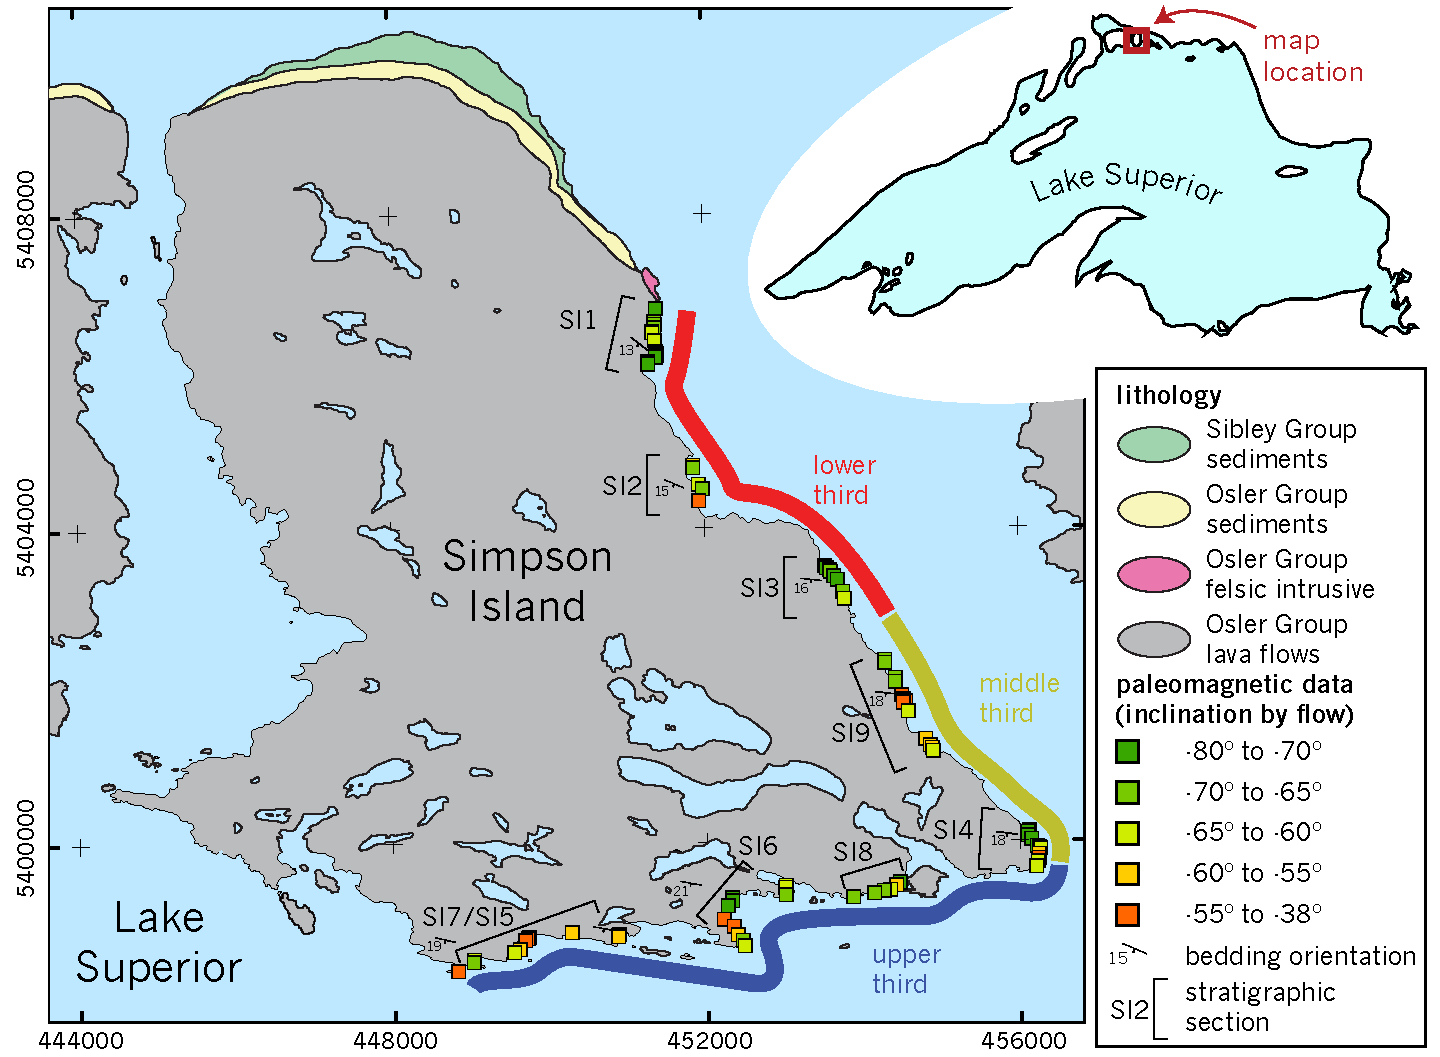
\includegraphics[width=\textwidth]{2014_Osler_Figures/Simpson_Island_Map.pdf}
\caption{Geological map of Simpson Island in the Lake Superior Archipelago with studied stratigraphic sections and lava flows shown. Data from flows are color-coded by inclination. The lava flows of the Osler Volcanic Group are tilted such that more southward flows are higher in the stratigraphy. The lower, middle and upper thirds divisions of the stratigraphic succession that are used in the text and in Figure \ref{fig:summary} are shown. The inset map shows the location of the geological map.}
\label{fig:map}
\end{figure}

\begin{figure}
\noindent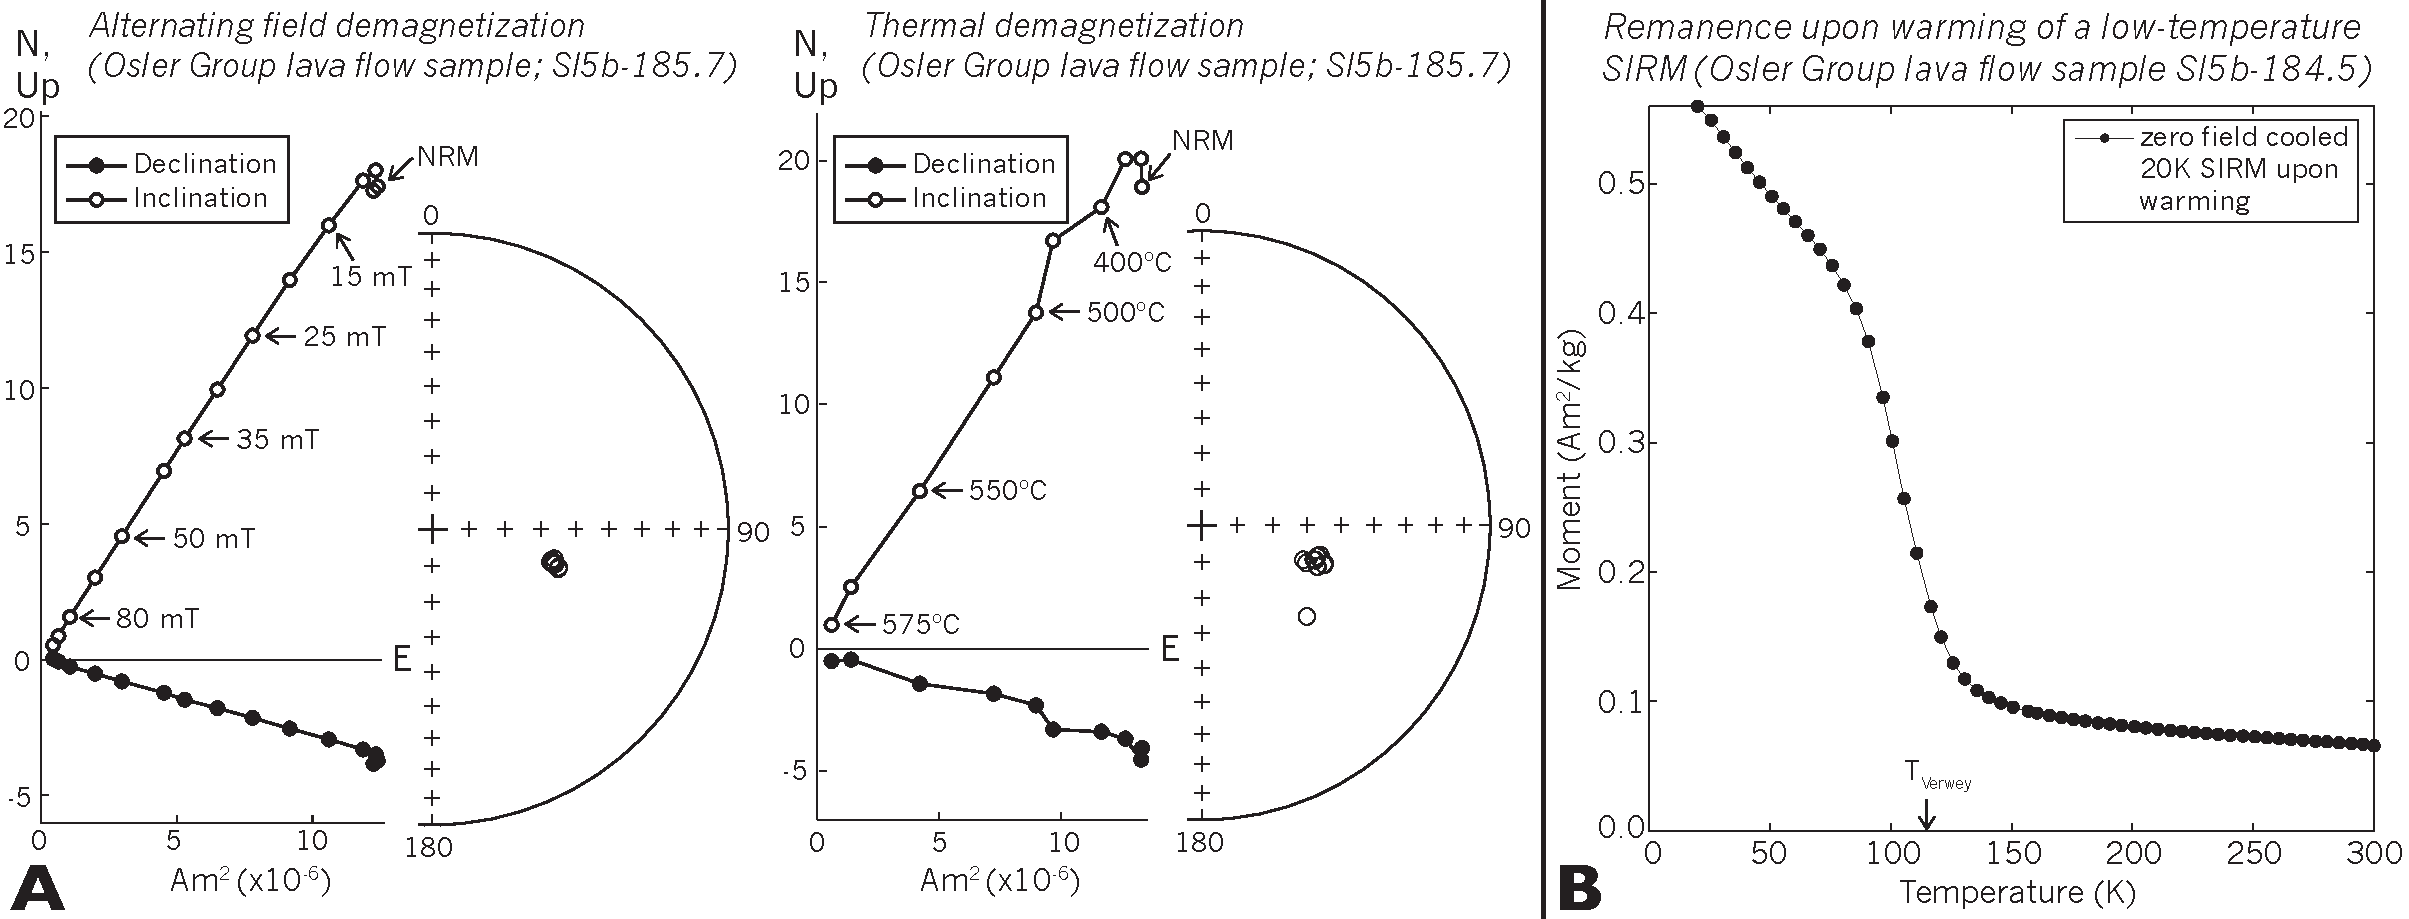
\includegraphics[width=\textwidth]{2014_Osler_Figures/PmagRockmag.pdf}
\caption{A) Paleomagnetic data for basaltic lava flow sample SI5b-185.7. Alternating field and thermal demagnetization data are shown for sister specimens of this sample in vector component and equal area diagrams. These data reveal a dominantly single-component remanence with both demagnetization protocols isolating the same direction. B) Low temperature demagnetization data from a sample in the same lava flow wherein a saturating isothermal remanent magnetization (SIRM) was imposed at 20K after cooling in a zero field. Subsequent warming of this remanence led to significant demagnetization across temperatures characteristic of the Verwey transition indicating that the magnetic mineralogy of the sample is dominated by low-titanium magnetite.}
\label{fig:pmagrockmag}
\end{figure}

\begin{figure}
\noindent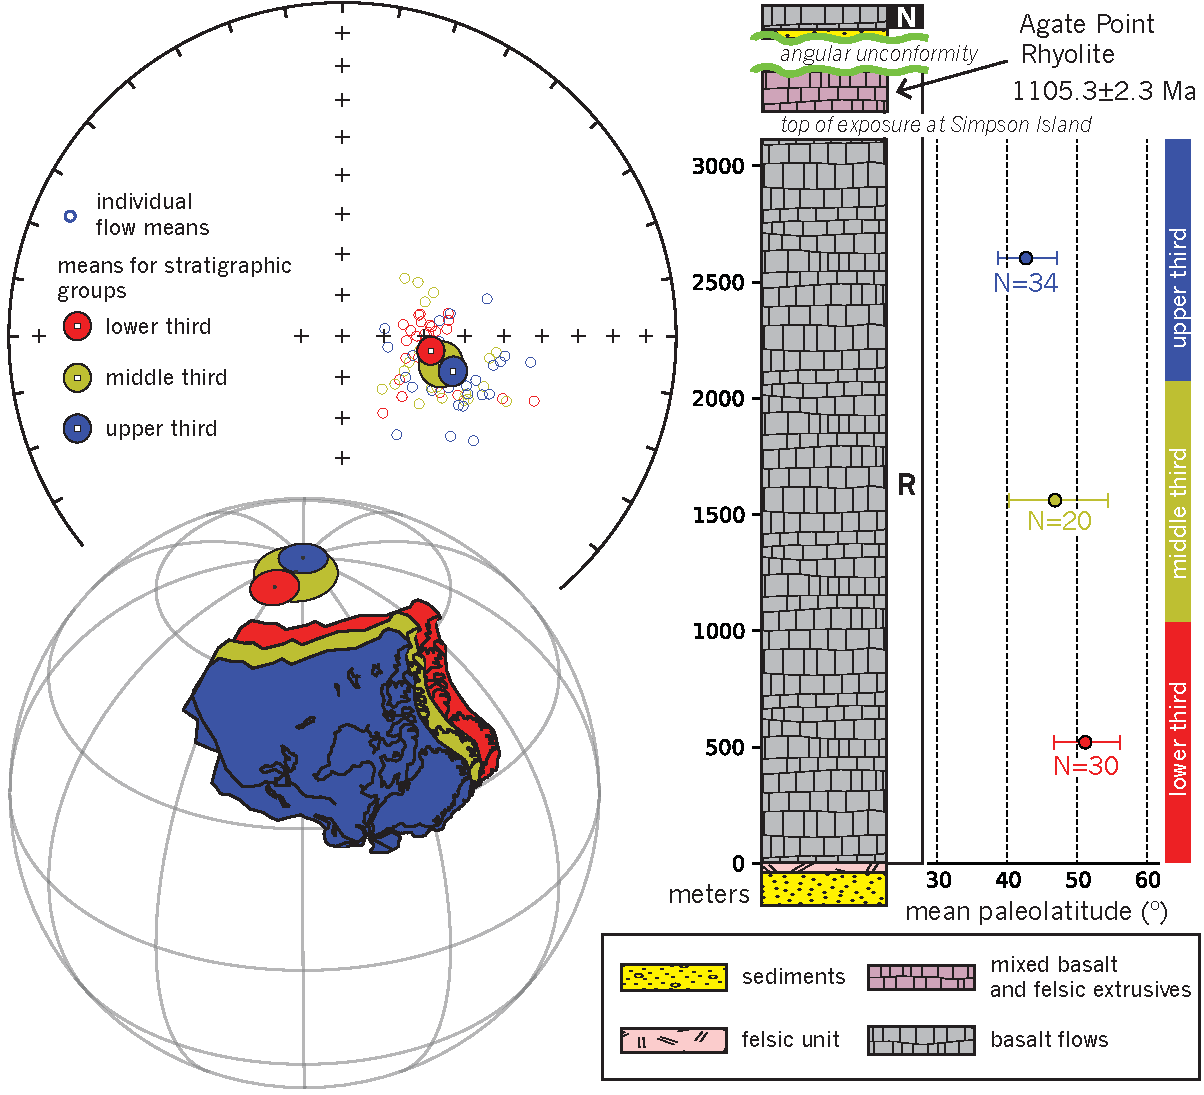
\includegraphics[width=0.8\textwidth]{2014_Osler_Figures/OslerStrat&EA.pdf}
\caption{Summary of paleomagnetic data from the Simpson Island exposure of the Osler Volcanic Group. The equal area plot shows the mean directions for each of the individual studied flows (N=84). All studied flows are of reverse polarity such that the plotted directions are in the upper hemisphere of the projection. Means are calculated and plotted on the equal area plot with $\alpha_{95}$ confidence ellipses for flows in the lower third (red; Dec=99.3, Inc=-68.0, $\alpha_{95}$=3.4, N=30), the middle third (yellow; Dec=105.9, Inc=-64.9, $\alpha_{95}$=5.9, N=20) and upper third (blue; Dec=107.6, Inc=-61.6, $\alpha_{95}$=3.5, N=34) of the stratigraphy. The mean paleolatitudes for these portions of the stratigraphy calculated from the Fisher means are also shown on the simplified composite stratigraphy with corresponding 2$\sigma$ error bars. The paleogeographic reconstruction shows Laurentia's progressive equatorward motion as constrained by the poles from each of the stratigraphic groupings.}
\label{fig:summary}
\end{figure}


%
% ---------------
% EXAMPLE TABLE
%
%\begin{table}
%\caption{Time of the Transition Between Phase 1 and Phase 2\tablenotemark{a}}
%\centering
%\begin{tabular}{l c}
%\hline
% Run  & Time (min)  \\
%\hline
%  $l1$  & 260   \\
%  $l2$  & 300   \\
%  $l3$  & 340   \\
%  $h1$  & 270   \\
%  $h2$  & 250   \\
%  $h3$  & 380   \\
%  $r1$  & 370   \\
%  $r2$  & 390   \\
%\hline
%\end{tabular}
%\tablenotetext{a}{Footnote text here.}
%\end{table}

% See below for how to make sideways figures or tables.

\end{document}

%%%%%%%%%%%%%%%%%%%%%%%%%%%%%%%%%%%%%%%%%%%%%%%%%%%%%%%%%%%%%%%

More Information and Advice:

%% ------------------------------------------------------------------------ %%
%
%  SECTION HEADS
%
%% ------------------------------------------------------------------------ %%

% Capitalize the first letter of each word (except for
% prepositions, conjunctions, and articles that are
% three or fewer letters).

% AGU follows standard outline style; therefore, there cannot be a section 1 without
% a section 2, or a section 2.3.1 without a section 2.3.2.
% Please make sure your section numbers are balanced.
% ---------------
% Level 1 head
%
% Use the \section{} command to identify level 1 heads;
% type the appropriate head wording between the curly
% brackets, as shown below.
%
%An example:
%\section{Level 1 Head: Introduction}
%
% ---------------
% Level 2 head
%
% Use the \subsection{} command to identify level 2 heads.
%An example:
%\subsection{Level 2 Head}
%
% ---------------
% Level 3 head
%
% Use the \subsubsection{} command to identify level 3 heads
%An example:
%\subsubsection{Level 3 Head}
%
%---------------
% Level 4 head
%
% Use the \subsubsubsection{} command to identify level 3 heads
% An example:
%\subsubsubsection{Level 4 Head} An example.
%
%% ------------------------------------------------------------------------ %%
%
%  IN-TEXT LISTS
%
%% ------------------------------------------------------------------------ %%
%
% Do not use bulleted lists; enumerated lists are okay.
% \begin{enumerate}
% \item
% \item
% \item
% \end{enumerate}
%
%% ------------------------------------------------------------------------ %%
%
%  EQUATIONS
%
%% ------------------------------------------------------------------------ %%

% Single-line equations are centered.
% Equation arrays will appear left-aligned.

Math coded inside display math mode \[ ...\]
 will not be numbered, e.g.,:
 \[ x^2=y^2 + z^2\]

 Math coded inside \begin{equation} and \end{equation} will
 be automatically numbered, e.g.,:
 \begin{equation}
 x^2=y^2 + z^2
 \end{equation}

% IF YOU HAVE MULTI-LINE EQUATIONS, PLEASE
% BREAK THE EQUATIONS INTO TWO OR MORE LINES
% OF SINGLE COLUMN WIDTH (20 pc, 8.3 cm)
% using double backslashes (\\).

% To create multiline equations, use the
% \begin{eqnarray} and \end{eqnarray} environment
% as demonstrated below.
\begin{eqnarray}
  x_{1} & = & (x - x_{0}) \cos \Theta \nonumber \\
        && + (y - y_{0}) \sin \Theta  \nonumber \\
  y_{1} & = & -(x - x_{0}) \sin \Theta \nonumber \\
        && + (y - y_{0}) \cos \Theta.
\end{eqnarray}

%If you don't want an equation number, use the star form:
%\begin{eqnarray*}...\end{eqnarray*}

% Break each line at a sign of operation
% (+, -, etc.) if possible, with the sign of operation
% on the new line.

% Indent second and subsequent lines to align with
% the first character following the equal sign on the
% first line.

% Use an \hspace{} command to insert horizontal space
% into your equation if necessary. Place an appropriate
% unit of measure between the curly braces, e.g.
% \hspace{1in}; you may have to experiment to achieve
% the correct amount of space.


%% ------------------------------------------------------------------------ %%
%
%  EQUATION NUMBERING: COUNTER
%
%% ------------------------------------------------------------------------ %%

% You may change equation numbering by resetting
% the equation counter or by explicitly numbering
% an equation.

% To explicitly number an equation, type \eqnum{}
% (with the desired number between the brackets)
% after the \begin{equation} or \begin{eqnarray}
% command.  The \eqnum{} command will affect only
% the equation it appears with; LaTeX will number
% any equations appearing later in the manuscript
% according to the equation counter.
%

% If you have a multiline equation that needs only
% one equation number, use a \nonumber command in
% front of the double backslashes (\\) as shown in
% the multiline equation above.

%% ------------------------------------------------------------------------ %%
%
%  SIDEWAYS FIGURE AND TABLE EXAMPLES
%
%% ------------------------------------------------------------------------ %%
%
% For tables and figures, add \usepackage{rotating} to the paper and add the rotating.sty file to the folder.
% AGU prefers the use of {sidewaystable} over {landscapetable} as it causes fewer problems.
%
% \begin{sidewaysfigure}
% \includegraphics[width=20pc]{samplefigure.eps}
% \caption{caption here}
% \label{label_here}
% \end{sidewaysfigure}
%
%
%
% \begin{sidewaystable}
% \caption{}
% \begin{tabular}
% Table layout here.
% \end{tabular}
% \end{sidewaystable}
%
%

